\label{sec:exp1}
En la primera parte de este laboratorio, se propuso determinar los valores de los componentes resistivo e inductivo de un inductor real. Como se explico en la sección~\ref{sec:Ind}, un inductor real pose un componente resistivo, en contraposición con su modelo idealizado. Para medir la resistencia se alimento una bobina con una señal triangular, como se explayo previamente, es de esperar que la señal resultante a los bornes de la bobina sea una suma de la derivada de la función de entrada (en este caso una señal cuadrada) y la misma señal triangular atenuada, esto debido a los distintos elementos que componen este inductor. Entonces midiendo las amplitudes de las distintas secciones de la señal de salida es posible estimar los valores de los distintos componentes.

\begin{figure}[H]
    \centering
    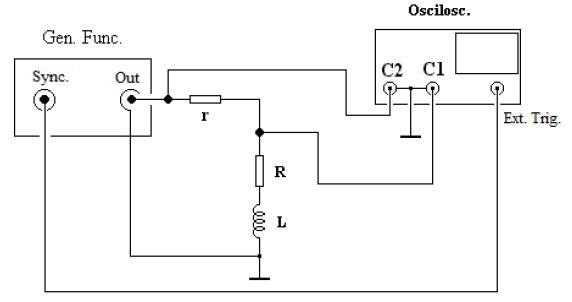
\includegraphics[width=0.7\linewidth]{Imagenes/exp1.PNG}
    \caption{Circuito experimento 1}
    \label{fig:exp1}
\end{figure}

Recordando la ecuación de aproximación a un inductor (\ref{eq:InducGn}):
\begin{equation*}
    V_{(\mathscr{s})}=I_{(\mathscr{s})}[r_l+\mathscr{s}L]
\end{equation*}


Se puede observar que la señal de entrada debe ser una señal de corriente para poder generar la señal de salida deseada. Esto se pude conseguir a través del uso de un generador de funciones común y una resistencia mayor a la del inductor. Planteando el circuito:
\begin{figure}[H]
    \centering
    \begin{circuitikz}[scale=1,every node/.style={transform shape},style=american]
\draw (0,2)to[open,v=$v_i$,o-o](0,-2)--(3,-2)to[inductor=$L$](3,0)to[R=$r_l$](3,2) (0,2)to[R=$R_g$,i=$i_{(t)}$](3,2);
\draw[line width=0.7pt,dashed] (2.3,-1.8)rectangle(3.3,1.8);
\draw (3.7,0)to[open,v=$v_L$](3.7,-2)  (3.7,2)to[open,v=$v_r$](3.7,0);
\end{circuitikz}

    \caption{Circuito equivalente del experimento 1}
    \label{fig:CircExp1}
\end{figure}
Tomando en cuenta que el circuito no fue excitado previamente y no posee carga alguna en el momento previo al experimento, se puede resolver que:
\begin{equation}
    \begin{aligned}
            v_{i(t)}=i_{(t)}(R_g+r_l)+L\cdot\frac{d~i_{(t)}}{dt}\llrah{\mathcal{L}} V_{(\mathscr{s})}&=I_{(\mathscr{s})}[R_g+r_l+\mathscr{s}L]\\
            I_{(\mathscr{s})}=&\frac{V_{(\mathscr{s})}}{R_g+r_l+\mathscr{s}L}\\
            I_{(\mathscr{s})}=&\frac{1}{L}\cdot\frac{V_{(\mathscr{s})}}{\mathscr{s}+\frac{R_g+r_l}{L}}\\
    \end{aligned}
\end{equation}
Para poder comprobar el valor necesario para obtener una señal de corriente estable se planteo excitar el circuito con una función escalón de tensión ($V_{i\mathscr{s}}=V_p/\mathscr{s}$):
\begin{equation}\label{eq:finepx3}
    \begin{aligned}
            I_{(\mathscr{s})}=&\frac{1}{L}\cdot\frac{1}{\mathscr{s}+\frac{R_g+r_l}{L}}\cdot \frac{V_p}{\mathscr{s}}\\
            I_{(\mathscr{s})}=&\frac{V_p}{L}(\frac{L/(R_g+r_l)}{\mathscr{s}}-\frac{L/(R_g+r_l)}{\mathscr{s}+\frac{R_g+r_l}{L}})\llrah ~i_{(t)}=\frac{V_p}{R_g+r_l}\cdot(1-e^{-t\frac{R_g+r_l}{L}})
    \end{aligned}
\end{equation}
Según este análisis, se puede deducir, que la señal de salida $i_{(t)}$ depende de la expresión $V_p/(R_g+r_l)$ (despreciando el régimen transitorio del circuito). Estableciendo que la señal debe tener una una variación de no menos del $0.5\%$ cuando se coloque alguna carga y planteando una resistencia interna del inductor de unos $500\Omega$ podemos determinar que la resistencia de entrada debe ser igual a $R_g=100k\Omega$.

Ya determinada la resistencia de entrada, se planteo el análisis del circuito equivalente de la bobina de la siguiente manera. Si se excita al circuito con una señal triangular ($A/(T/2)\cdot t$) ,es de esperar que la señal a los bornes de la bobina se la suma entre una señal cuadrada, debido a el efecto derivador de la inductancia y la misma señal triangular reducida por la resistencia $r_l$. Entonces se puede plantear lo siguiente:
\begin{figure}[H]
    \centering
    \begin{minipage}{0.49\textwidth}
        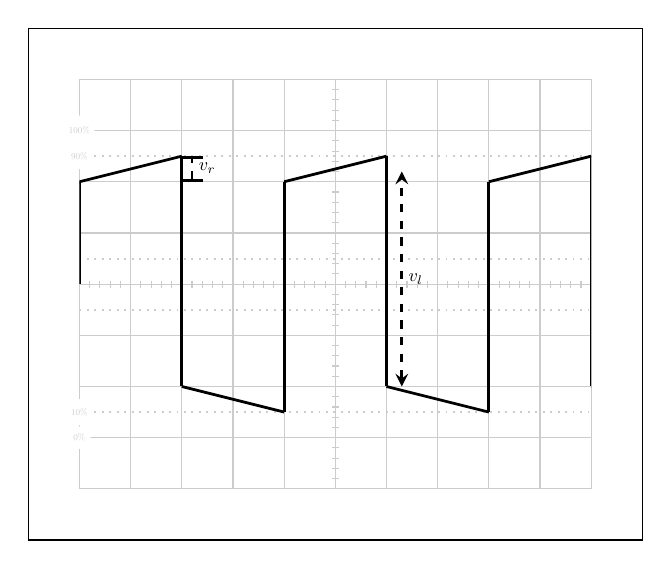
\begin{tikzpicture}[scale=0.65,every node/.style={transform shape}]
\def\res{0.5};%EscalaTemporal señal 1
\def\ind{1};%EscalaTemporal señal 2
\def\scalVa{1};%EscalaVertical señal 1
\def\frec{5};%EscalaVertical señal 2
\def\offseta{0};%Nivel de offset de la señal señal 1
\def\offsetb{};%Nivel de offset de la señal señal 2

%Lineas intermedias grilla
\foreach \x in {-5,-4.8,...,4.8,5}{
    \draw[gray!40,thin,shift={(\x,0)}] (0pt,2pt) -- (0pt,-2pt);
}
\foreach \y in {-4,-3.8,...,3.8,4}{
    \draw[gray!40,thin,shift={(0,\y)}] (2pt,0pt) -- (-2pt,0pt);
}
\foreach \a [evaluate={\y=\a*0.5}] in {-5,-1,1,5}{
    \draw[gray!40,line width=0.7pt,dotted] (-5,\y) -- (5,\y);
}

%Grilla
\draw[thin,gray!40] (-5,-4) grid (5,4);
\node[fill=white,text=gray!40,circle,scale=0.5] at (-5,3) {$100\%$};
\node[fill=white,text=gray!40,circle,scale=0.5] at (-5,2.5) {$90\%$};
\node[fill=white,text=gray!40,circle,scale=0.5] at (-5,-2.5) {$10\%$};
\node[fill=white,text=gray!40,circle,scale=0.5] at (-5,-3) {$0\%$};
\draw[black] (-6,-5) rectangle(6,5);

%Señal 1
\clip (-5,-4) rectangle (5,4);
\foreach [evaluate={\a=(-5+(4*\c))}][evaluate={\b=-3+(4*\c)}]\c in{0,...,2}{
    \draw[line width=1pt](\a,2)--(\a+2,2.5){};
    \draw[line width=1pt](\b,-2)--(\b+2,-2.5){};
    \draw[line width=1pt](\a+2,2.5)--(\b,-2) (\b+2,-2.5)--(\b+2,0) (\a,0)--(\a,2);

}
\draw[line width=1pt,dashed,stealth-stealth](1.3,-2)--(1.3,2.2) node[midway,right]{$v_l$};
\draw[line width=1pt,dashed,stealth-stealth,|-|](-2.8,2)--(-2.8,2.5)node[anchor=north west]{$v_r$};
\end{tikzpicture}
%\caption*{Un osciloscopio}
%\draw [mblk]plot[smooth,samples=100,domain=(0:1)](\x,{\scalVa*(1/\frec-(2*\res)/\frec*\x-(2*\ind)/\frec)+\offseta});
%\draw[line width=1pt,mdblu](-5,{2*\scalVa*\ind)/\frec})--(5,{2*\scalVa*\ind)/\frec}) (-5,{-2*\scalVa*\ind)/\frec})--(5,{-2*\scalVa*\ind)/\frec});
%Señal 2
%\draw [mblk]plot[smooth,samples=100,domain=(0:1)](\x,{\scalVa*(1/\frec-(2*\res)/\frec*\x-(2*\ind)/\frec)+\offseta});
%\draw[line width=1pt,mdblu](-5,{2*\scalVa*\ind)/\frec})--(5,{2*\scalVa*\ind)/\frec}) (-5,{-2*\scalVa*\ind)/\frec})--(5,{-2*\scalVa*\ind)/\frec});
        \label{fig:enter-label}
    \end{minipage}
    \begin{minipage}{0.49\textwidth}
        \begin{equation}\label{eq:Senexp1}
        \begin{aligned}
            v_{ind}&=r_l\cdot i_{(t)}+2L\frac{V_p}{T}\\
            \\
        v_{ind}&\begin{cases}
            r_l=\frac{v_r}{V_p}\\
            \\
            L=\frac{v_l}{2\cdot V_p \cdot f}
        \end{cases}
        \end{aligned}
    \end{equation}
\end{minipage}
\caption{Análisis del circuito equivalente de una bobina}
\end{figure}


\unsubsubsection{Mediciones}
Se procedió a excitar el circuito con una señal de tensión triangular de amplitud $V_{pp}=20$ y distintas frecuencias para observar el comportamiento lineal en frecuencia que pose el inductor.
Los valores nominales de la bobina utilizada en el experimento fueron los siguientes:

\begin{equation*}
    R_{nom} = 200 ~\Omega  
    \hspace{2cm}
    L_{nom} = 1.5 ~H
\end{equation*}

Realizando las mediciones correspondiente y utilizando las ecuaciones \ref{eq:Senexp1}.a y\ref{eq:Senexp1}.b se obtuvieron los siguientes datos.
\begin{figure}[H]
    \centering
    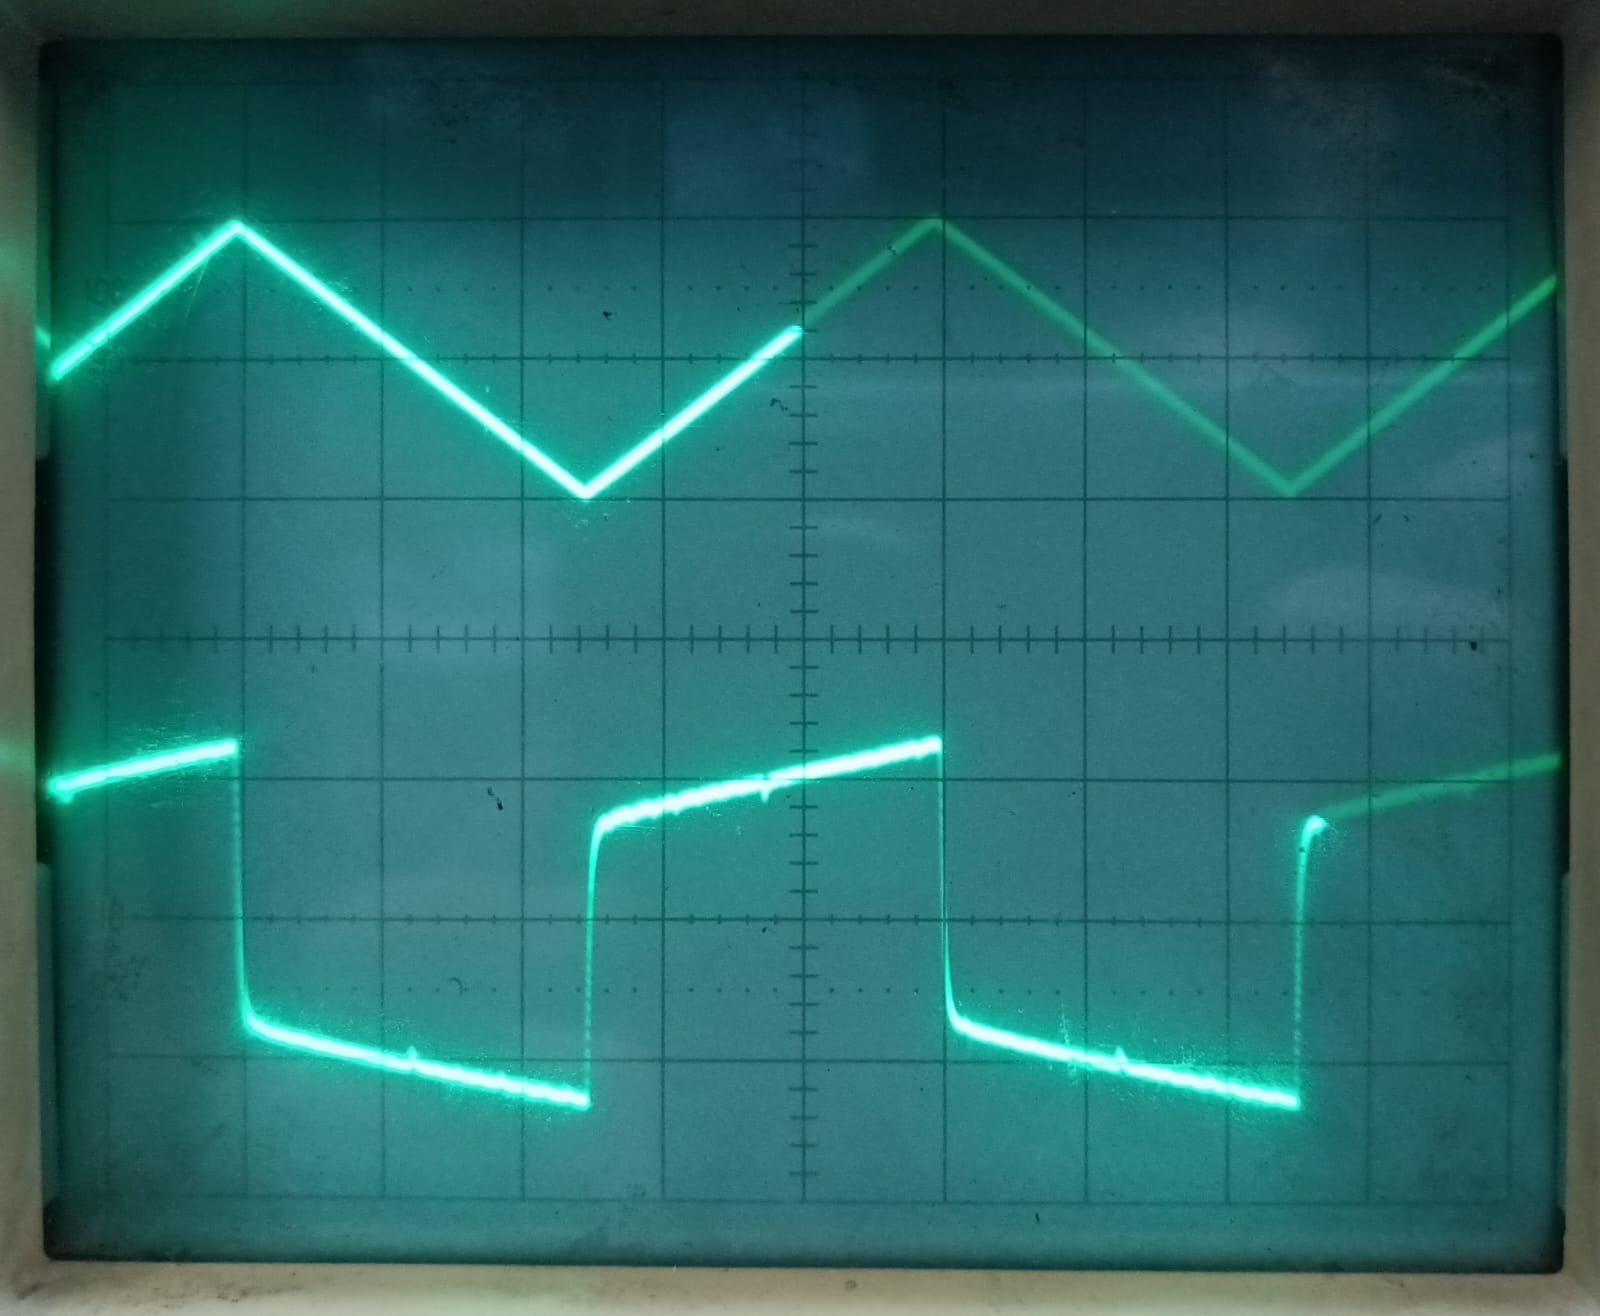
\includegraphics[width=0.6\textwidth,trim={0 0 0 0},clip]{Imagenes/MedExp1.jpeg}
    \caption{Medición de la señal de entrada vs salida del experimento 1}
\end{figure}

\begin{table}[H]
    \centering
    \begin{tabular}{|c|c|c|c|}
    \hline
        $f$ & $f_1 = 50~Hz$ & $f_2 = 100~Hz$ & $f_3 = 200~Hz$ \\
    \hline
        $r$ & \multicolumn{3}{c|}{$100~k\Omega$}\\
    \hline
        $I_{RMS}~[\mu A]$ & 52.1 & 52.17 & 55.11\\
        $I_{pp}~[\mu A]$ & 180.48 & 180.72 & 190.9\\
    %\hline
        $e_{pp} = 2 e_L ~[mV]$ & 100 & 200 & 400  \\
    %\hline    
        $e_R~[mV]$ & 48 & 56 & 65,17 \\
    %\hline    
        $L~[H]$ & 2.77 & 2.767 & 2.619 \\
    %\hline    
        $R~[\Omega]$ & 265.957 & 309.87 & 341.383 \\
    \hline    
    
        \end{tabular}
        \def\tablename{Tabla} 
        \caption{Tabla de parámetros a distintas frecuencias}
        \label{tab:exp1}
\end{table}

Como se puede observar los valores de inductancia varían entre las frecuencias de manera lineal, dando una media de $L_m=2.767~H$, siguiendo el comportamiento esperado. Lo que discrepa en estas mediciones con el modelo matemático planteado  es la variación del valor del componente resistivo. Se planteo la hipótesis de que esta variación se debe al efecto de los flujos magnéticos del circuito magnético debido a el núcleo de hierro que compone a la bobina. Debido a la falta de información sobre otros fenómenos que pueden ocasionar este comportamiento, se concluyo que esta es la razón mas factible que explica este efecto.

\unsubsubsection{Comprobación}
Se utilizo un medidor RLC para comprobar la precisión de las estimaciones:
\begin{figure}[H]
    \begin{minipage}{0.49\textwidth}
    \centering
    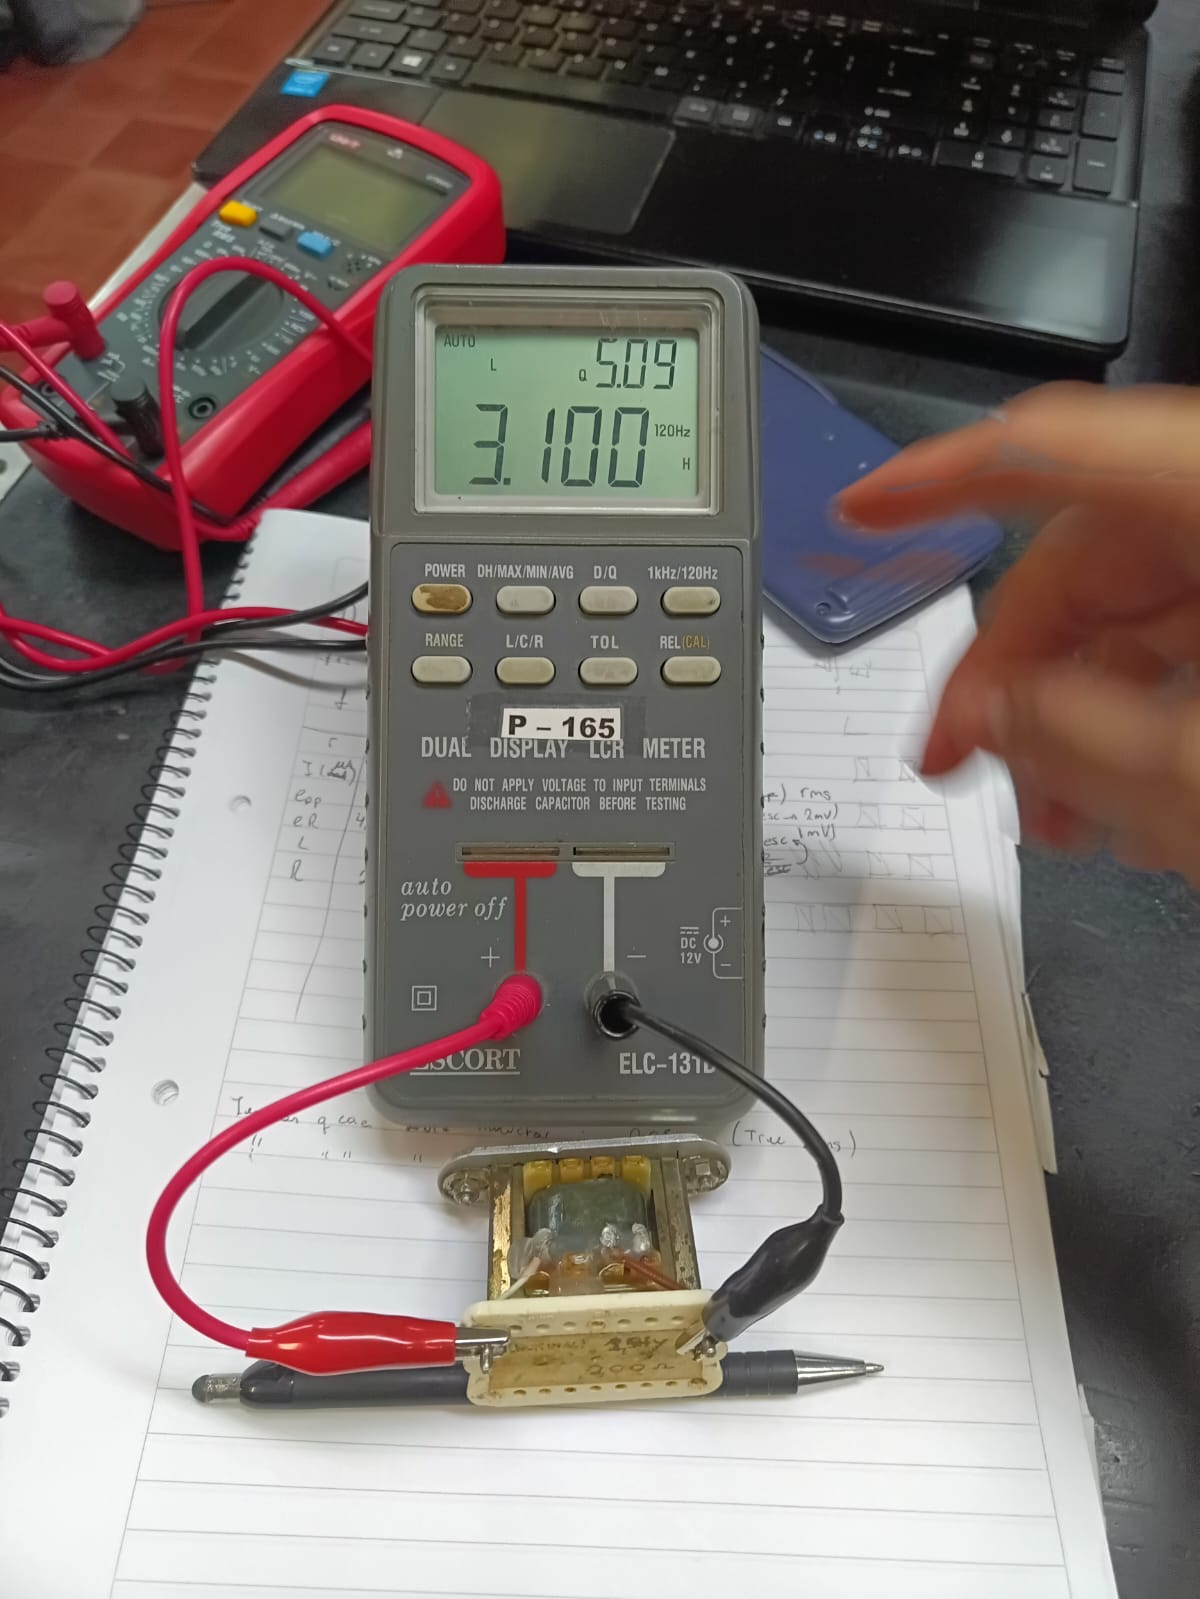
\includegraphics[width=0.65\textwidth,trim={5cm 5cm 12cm 10cm},clip]{Imagenes/MedInd1Exp1.jpeg}
    \caption{Medición en frec. de $F=120 Hz$}
    \end{minipage}
    \begin{minipage}{0.49\textwidth}
    \centering
    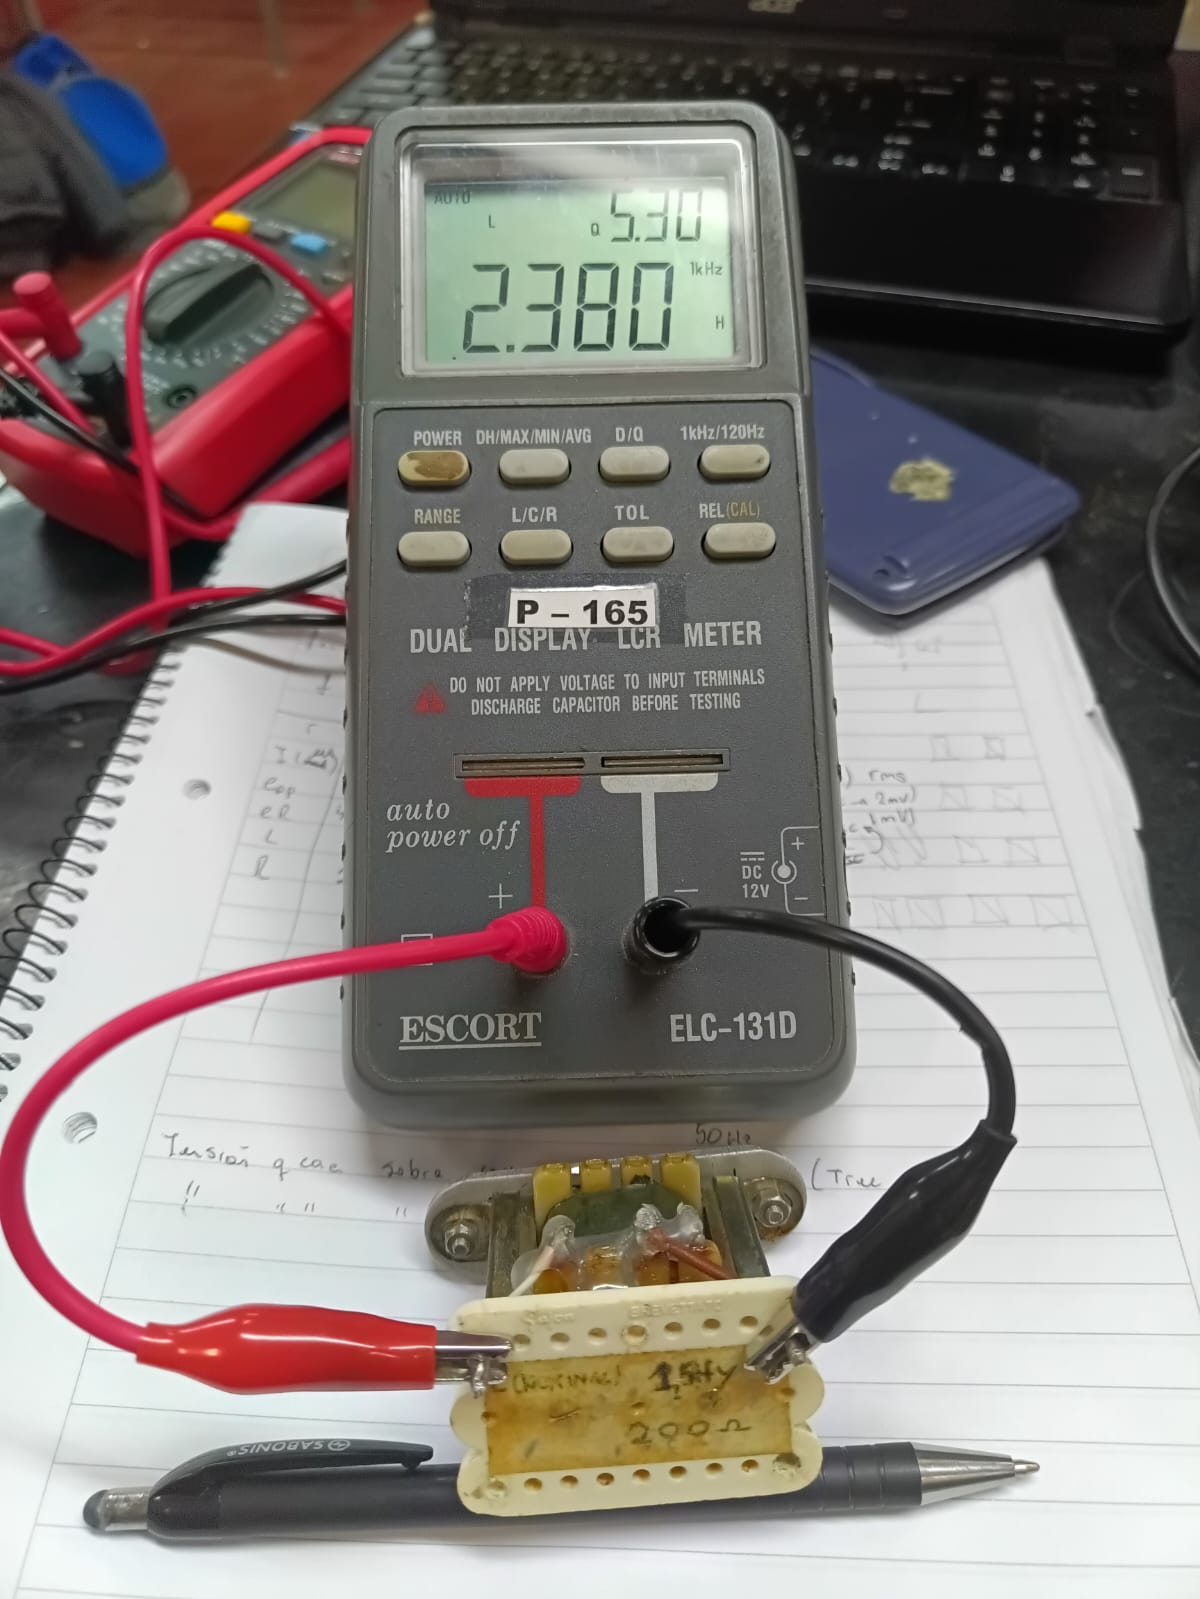
\includegraphics[width=0.715\textwidth,trim={2cm 0 5cm 4cm},clip]{Imagenes/MedInd2Exp1.jpeg}
    \caption{Medición en frec. de $F=1~Khz$}
    \end{minipage}
\end{figure}